\chapter{Propuesta de solución}

%=========================================================
%                                                         Problematica
%=========================================================
\section{Objetivos}
\noindent En esta sección se menciona el objetivo general y los objetivos especifícos, los cuales ayudarán a atacar la problemática.
\subsection{Objetivo General}
\noindent Desarrollar una aplicación web de apoyo para el Departamento Deportivo de la Escuela Superior de Cómputo (ESCOM) que permita la inscripción de interpolitécnicos, visualizar los eventos próximos y a su vez sea un espacio de información y difusión.
\subsection{Objetivos Especificos}
\begin{itemize}
	\item Implementar un mecanismo de validación del estatus académico del alumno. 
	\item Implementar un módulo para la generación de la cédula de inscripción con base en el formato oficial de interpolitécnicos deportivos. 
	\item Implementar un módulo de comunicación con la red social (Facebook). 
	\item Implementar un módulo de consulta de resultados de competencias.
\end{itemize}
\pagebreak

	%=========================================================
	%                                                         Marco teorico
	%=========================================================
	\section{Alcance de la solución}
	\noindent En la Figura \ref{arquitectura} se muestra la arquitectura de la aplicación web,
	\begin{figure}[hbt!]
		\centering
		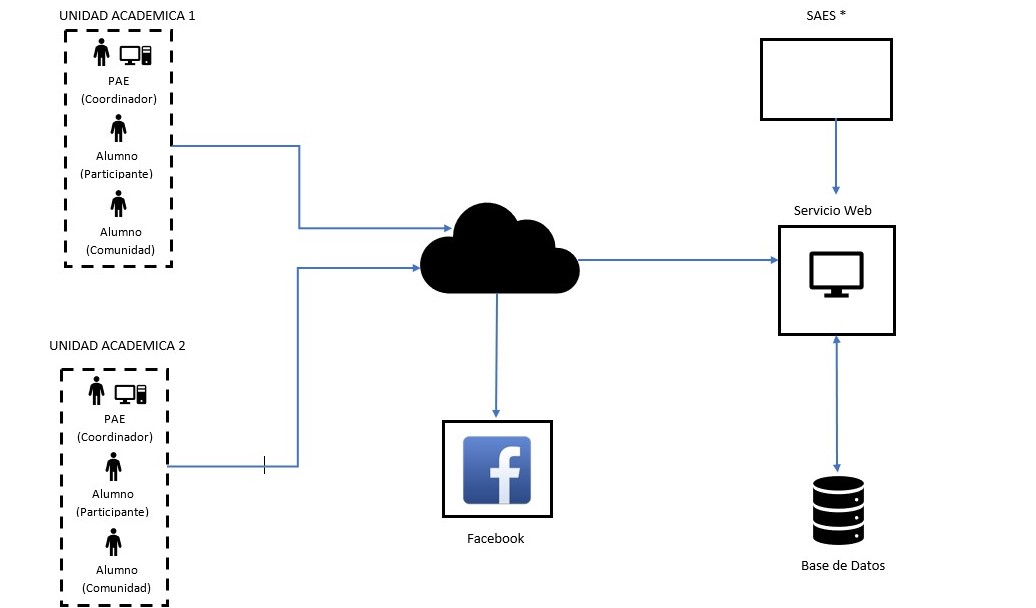
\includegraphics[width=10cm, height=6cm]{Imagenes/arquitectura}
		\caption{Arquitectura del sistema}
		\label{arquitectura}
	\end{figure}

	\noindent Como se puede observar, esta contempla su implementación en otras unidades académicas, sin embargo cabe mencionar que el Trabajo Terminal se enfocará particularmente en ESCOM con el objetivo de análisar, estudiar la aceptación del mismo, así como posibles mejoras.
	
	\noindet La aplicación esta involucrada por 3 usuarios, el Jefe de Departamento de Fomento Deportivo, el coordinador de Unidad Académica y el alumno. En esta cada uno tendrá distintos permisos y funciones dentro de la aplicación, el Jefe de Departamento de Fomento Deportivo será el encargado de publicar eventos deportivos, agregar nuevos deportes junto con las pruebas de los mismos, el coordinador de Unidad Académica se encargará de cerrar el proceso de inscripición a los eventos, generar el listado de los alumnos inscritos y el ingresar los resultados obtenidos por los participantes, finalmente el alumno podrá inscribirse en los eventos de su interés, así como consultar su historial de participaciones y los eventos actuales en los que está inscrito.
	
	
	%=========================================================
	%                                                         Analisis de factibilidad tecnica
	%=========================================================
	\section{Crawler}
	\label{crawler}
	\noindent Este código fue desarrollado con el lenguaje de programación JAVA y JSOUP, permitiendo la simulación de la interacción de una persona “navegando” en la red, este “web crawler” fue desarrollado con el propósito de encontrar un mecanismo de validación para comprobar si realmente eres alumno de la ESCOM, donde se iniciará sesión con los datos del usuario de la plataforma de la escuela llamado SAES pidiendo un usuario (Boleta del alumno), contraseña y una clave captcha que el servidor de la plataforma genera como un filtro para evitar la intrusión de “bots informáticos”.\\
	
	\begin{figure}[hbt!]
		\centering
		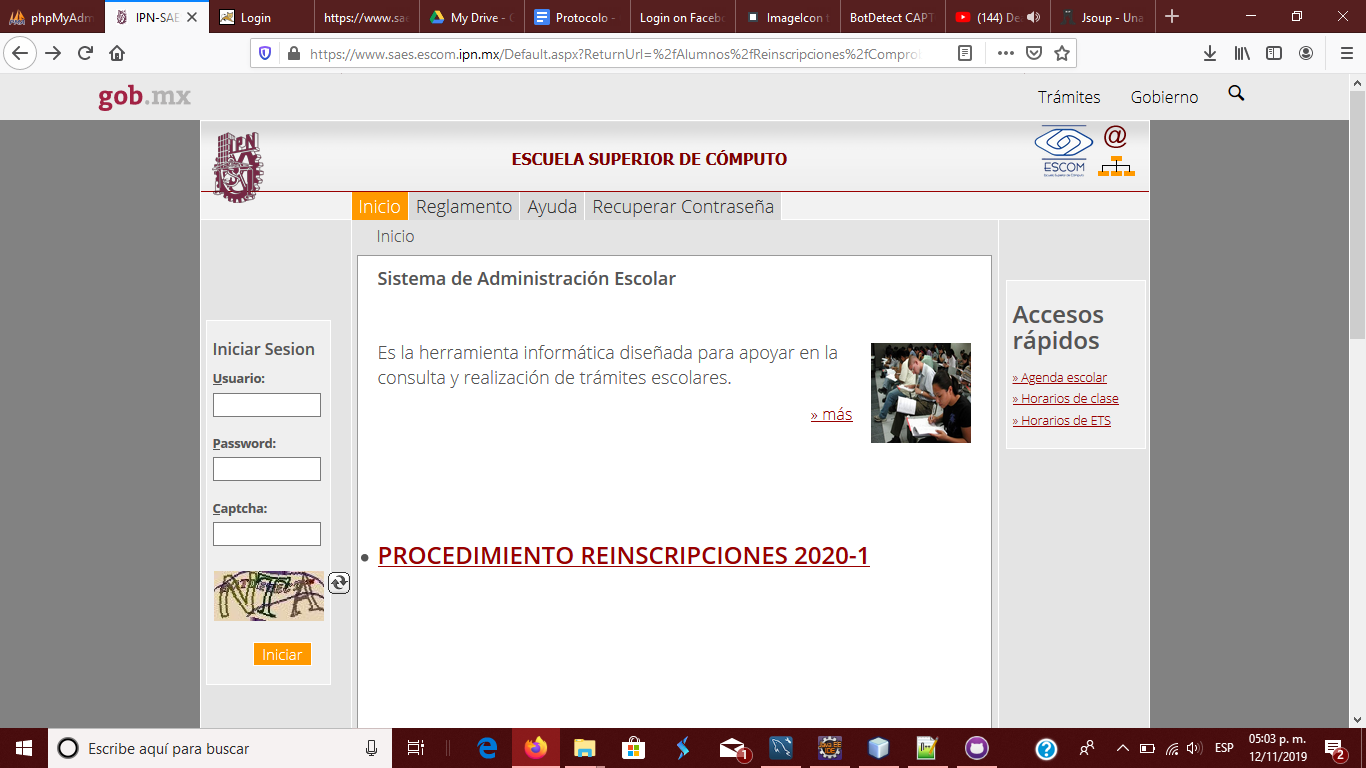
\includegraphics[width=10cm, height=6cm]{Imagenes/Crawler/SAES}
		\caption{Página del SAES Escom}
		\label{saes}
	\end{figure}
	
	\noindent Mediante las herramientas como JSOUP nos permite obtener información del HTML de cualquier página en la web, a excepción de la información generada con javascript pues las obtenciones de información son extraídas de manera estática y no de forma dinámica, o bien desde la lectura del HTML.\\
	\noindent Las pruebas de este código fueron realizadas durante los meses de enero del 2019 y octubre del mismo año. Utilizando así el siguiente código.
	\pagebreak
	
	\noindent Por inicio tenemos que importar las librerías de JSOUP para hacer uso de los métodos que se presentarán a continuación, además de crear datos públicos para los métodos de las clases java para utilizarlos posteriormente.\\
	\noindent Creamos la conexión con la página que queremos explorar y solicitar una respuesta de esta conexión realizada junto con las “cookies” generadas en esta respuesta, ya que estás nos darán pauta para mantenernos en la misma conexión con respecto a la solicitud de conexión hecha anteriormente. \\
	
	\begin{figure} [hbt!]
		\centering
		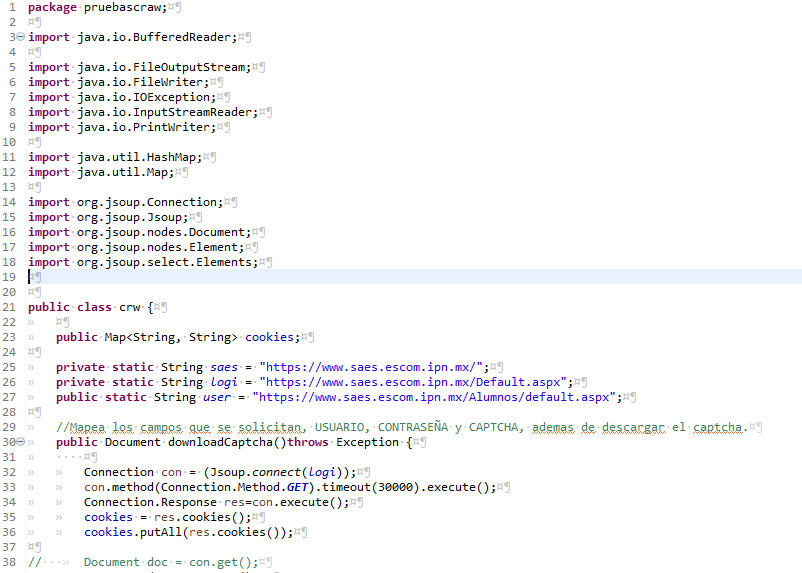
\includegraphics[width=10cm, height=6cm]{Imagenes/Crawler/Codigo1}
		\caption{Código desarrollado implementando el crawler.}
		\label{codigo1}
	\end{figure}
	
	\noindent Lo siguiente es realizar la exploración de los elementos del HTML en una variable de tipo “Document” de la página solicitada donde buscaremos el elemento por ID del CAPTCHA del HTML y así crear una imagen válida que fuese creada por el servidor, extrayendo la ubicación de la imagen para colocarla en una respuesta de conexión con la ruta de la imagen obtenida en la variable “a” y generarla de manera local utilizando “FileOutputStream”, el método creado es de tipo “Document” por lo tanto su salida es del mismo tipo. 
	\pagebreak
	
	\begin{figure} [hbt!]
		\centering
		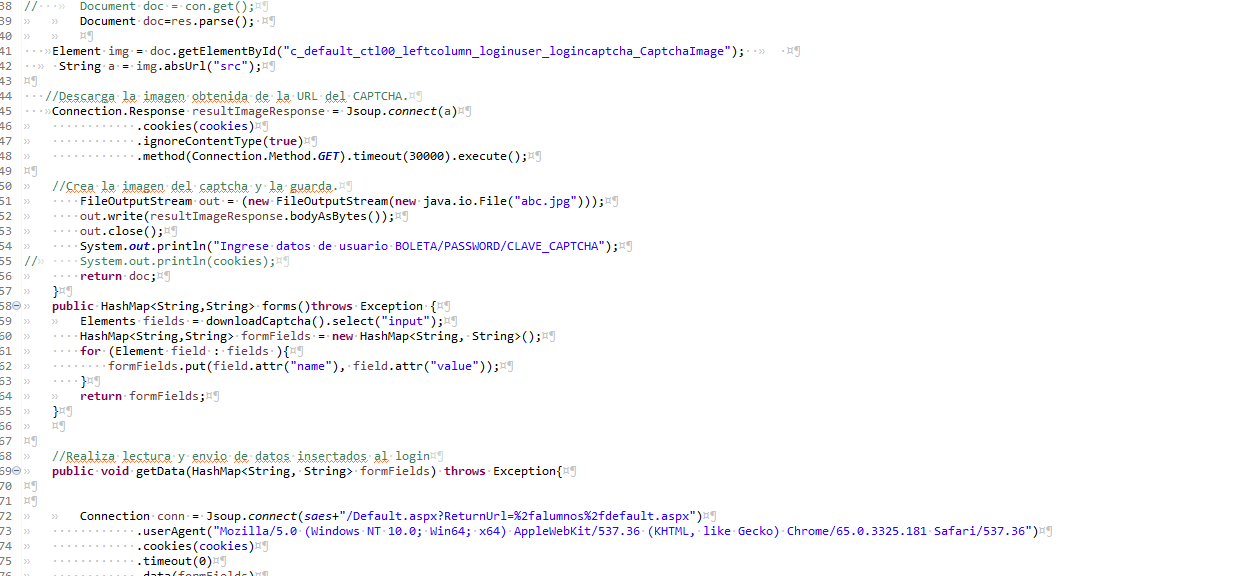
\includegraphics[width=10cm, height=8cm]{Imagenes/Crawler/Codigo2}
		\caption{Continuación de la implementación del crawler.}
		\label{codigo2}
	\end{figure}
	
	\noindent Una vez realizado este método procedemos a explorar los campos de inserción que existen en el HTML, para ello hacemos otra búsqueda de elementos en el HTML y definimos los datos que contienen estos elementos para su posterior inserción y uso de ellos mediante una variable de tipo “HashMap<String,String>” (todos los campos son de tipo cadena).\\
	
	\noindent Ahora la realización del método “getData(HashMap<String,String> formFields)” utilizaremos como parámetros los elementos de inserción explorados anteriormente insertándolos en nuestro método “POST”. Creamos la conexión a donde se debe redirigir la información del inicio de sesión, insertando también las cookies almacenadas en la previa conexión de la obtención del HTML de la página del SAES.\\
	
	\begin{figure} [hbt!]
		\centering
		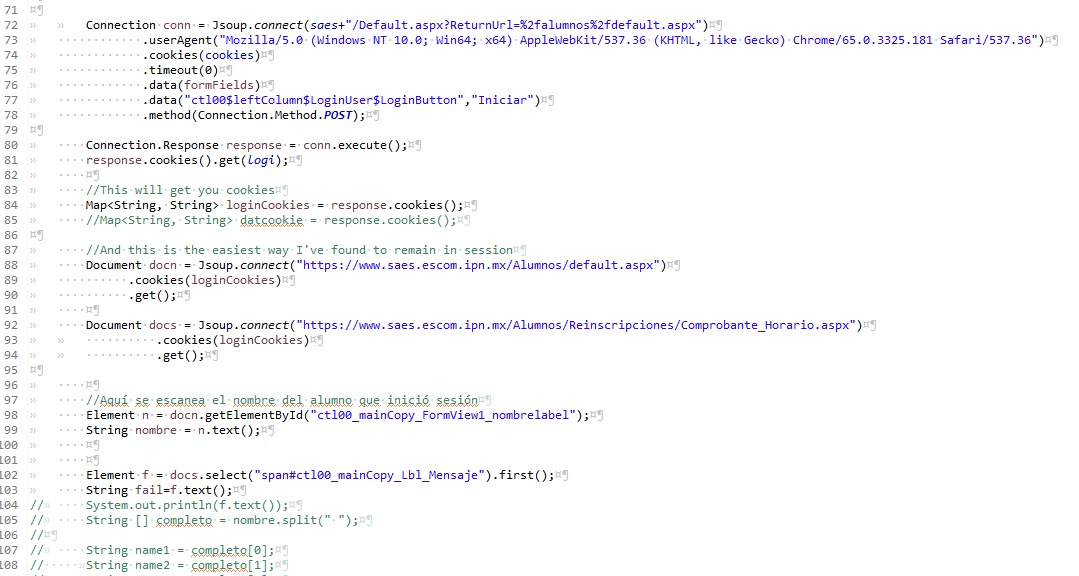
\includegraphics[width=10cm, height=8cm]{Imagenes/Crawler/Codigo3}
		\caption{Continuación implementación del crawler.}
		\label{codigo3}
	\end{figure}
	\pagebreak
	
	\noindent Si los datos ingresados son correctos se realizará una respuesta de la ruta solicitada en el POST insertando las cookies correspondientes a la conexión para comprobar la sesión del usuario en la plataforma, seguido de un mapeo del nuevo HTML donde se realizará la búsqueda por ID del campo donde se encuentre el nombre del alumno y un mensaje donde solo habrá texto si el usuario que haya iniciado sesión no estuviera inscrito.\\
	\noindent De lo anterior y siguiendo la condición de que el usuario que haya iniciado sesión esté o no inscrito dependerá si el texto buscado como “fail” sea nulo/vacío, en el caso de que no lo esté indicará que el alumno que haya iniciado sesión está “INSCRITO” indicando el nombre del alumno que corresponda a la boleta y usuario junto con un grupo al que pertenezca, en el caso de que “fail” no sea nulo/vacío se indicará que el alumno que corresponda a la boleta y usuario aparezca como “NO INSCRITO”. \\
	\begin{figure}[hbt!]
		\centering
		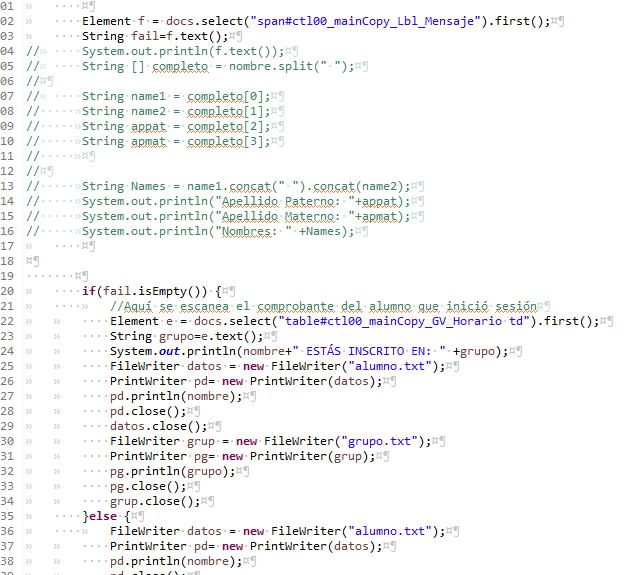
\includegraphics[width=10cm, height=8cm]{Imagenes/Crawler/Codigo4}
		\caption{Continuación implementación del crawler.}
		\label{codigo4}
	\end{figure}
	
	\noindent Finalmente se crean 3 archivos donde se almacena la información del usuario que haya iniciado sesión donde se inserta su nombre completo (alumno.txt), su grupo al que esté inscrito (grupo.txt) y el código HTML de la página donde se obtuvo toda esta información (respoinse.html).
	\pagebreak
	
	\begin{figure}[hbt!]
		\centering
		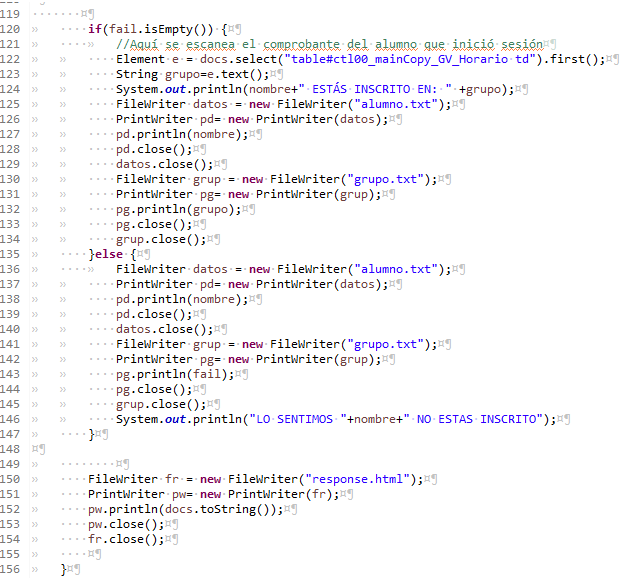
\includegraphics[width=10cm, height=6cm]{Imagenes/Crawler/Codigo5}
		\caption{Continuación de la implementación del crawler.}
		\label{codigo5}
	\end{figure}
	
	\noindent Una vez realizado esto necesitamos adjuntar estos métodos en 1 sola petición (o método) para realizar su ejecución e inserción de datos correspondientes a los que se necesitan.
	Como se hace en el método “run()”. \\
	
	\noindent Creamos un método donde se adjunta en 1 petición la ejecución de todos los métodos anteriores, y haremos la petición de los datos del inicio de sesión del SAES usando “readLine()” para hacer la lectura de estas seguido de la asignación de los campos que se escogen para insertar estas cadenas y reenviarlos al método “getData” donde los datos insertados serán los parámetros que servirán para la correcta funcionalidad del método “getData” y finalmente iniciar sesión.\\
	\begin{figure} [hbt!]
		\centering
		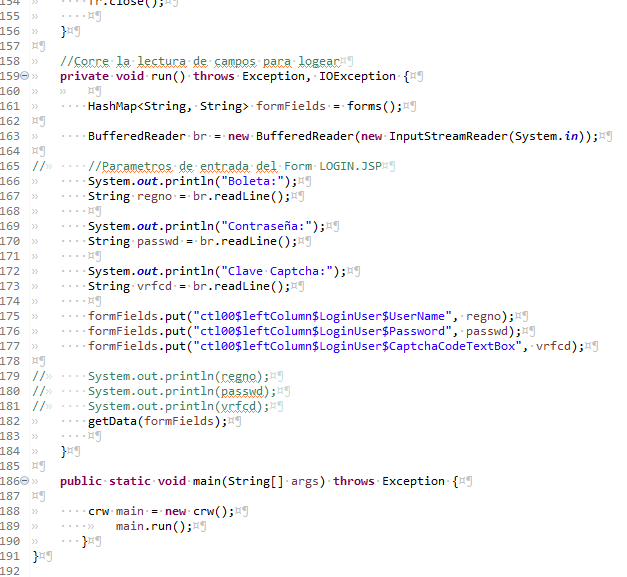
\includegraphics[width=10cm, height=8cm]{Imagenes/Crawler/Codigo6}
		\caption{Continuación implementación crawler.}
		\label{codigo6}
	\end{figure}
	\pagebreak
	\noindent Cabe mencionar que dicha plataforma está desarrollada con ASP.NET con un plugin detector de “bots” llamado “Captcha BotDetect”, donde desde el servidor se realiza la generación de credenciales correspondientes a la imagen que se muestre en la página como la conocemos.\\
	\textbf{“href="BotDetectCaptcha.ashx?get=layoutStyleSheet" ”}\\
	\begin{figure} [hbt!]
		\centering
		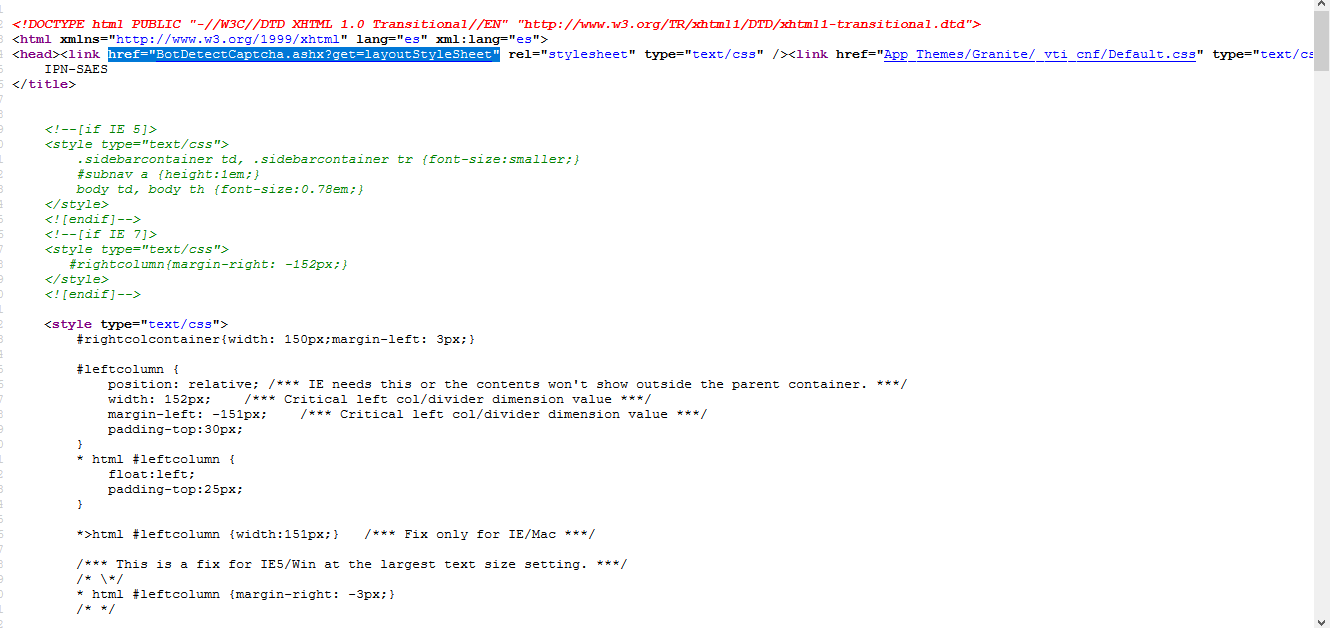
\includegraphics[width=10cm, height=6cm]{Imagenes/Crawler/ASP2}
		\caption{Inspección de estructura del SAES.}
		\label{asp2}
	\end{figure}
	
	\noindent Las peticiones de inicio de sesión se realizan directo al servidor y el servidor responde con un javascript donde redirecciona a la vista correspondiente si las credenciales de usuario y clave captcha son las correctas de acuerdo a la sesión de página en la que se encuentra.\\
	\textbf{“action="Default.aspx?ReturnUrl=\%2fAlumnos\%2fcambia\_clave.aspx" onsubmit="javascript:return WebForm\_OnSubmit();" ”}
	
	\begin{figure} [hbt!]
		\centering
		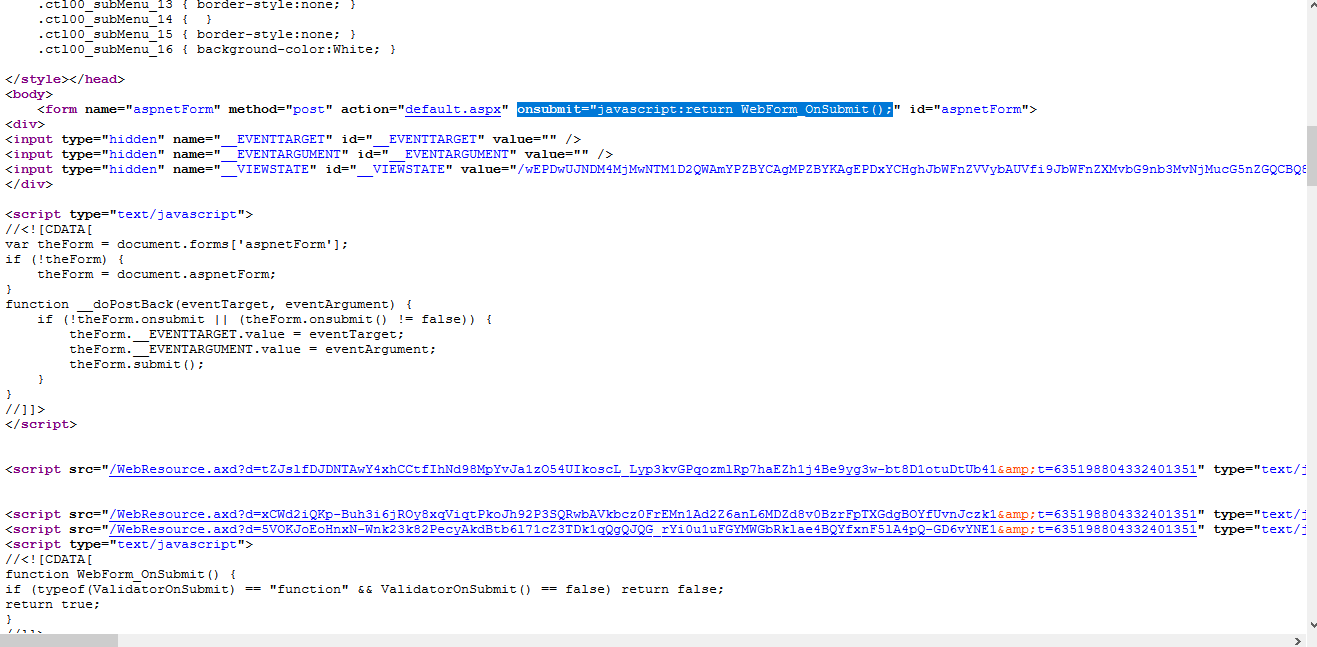
\includegraphics[width=10cm, height=6cm]{Imagenes/Crawler/ASP1}
		\caption{Inspección de estructura del SAES.}
		\label{asp1}
	\end{figure}
	\noindent Estos cambios se identificaron el día 15 de octubre del 2019.
	\pagebreak
	
	\textbf{POR EJEMPLO: CON USUARIO NO INSCRITO}\\
	\noindent Se inserta previamente la boleta y contraseña del alumno del SAES ESCOM.
	
	\begin{figure}[hbt!]
		\centering
		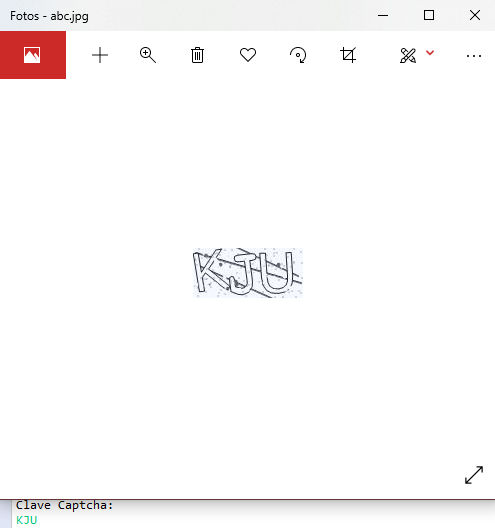
\includegraphics[width=10cm, height=5cm]{Imagenes/Crawler/ImagenloginNoinscrito}
		\caption{Captcha para alumno no inscrito.}
		\label{imagenloginnoinscrito}
	\end{figure}
	
	Se ingresa la clave captcha mostrada en la imagen “KJU”
	
	\begin{figure}[hbt!]
		\centering
		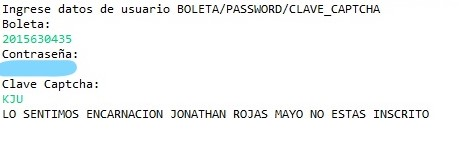
\includegraphics[width=10cm, height=5cm]{Imagenes/Crawler/Datosloginnoinscrito}
		\caption{Se ingresan los datos en el crawler.}
		\label{datosloginnoinscrito}
	\end{figure}
	\noindent Responde de acuerdo a la inscripción del alumno, para este caso el alumno NO ESTÁ INSCRITO.
	\pagebreak
	
	\begin{figure}[hbt!]
		\centering
		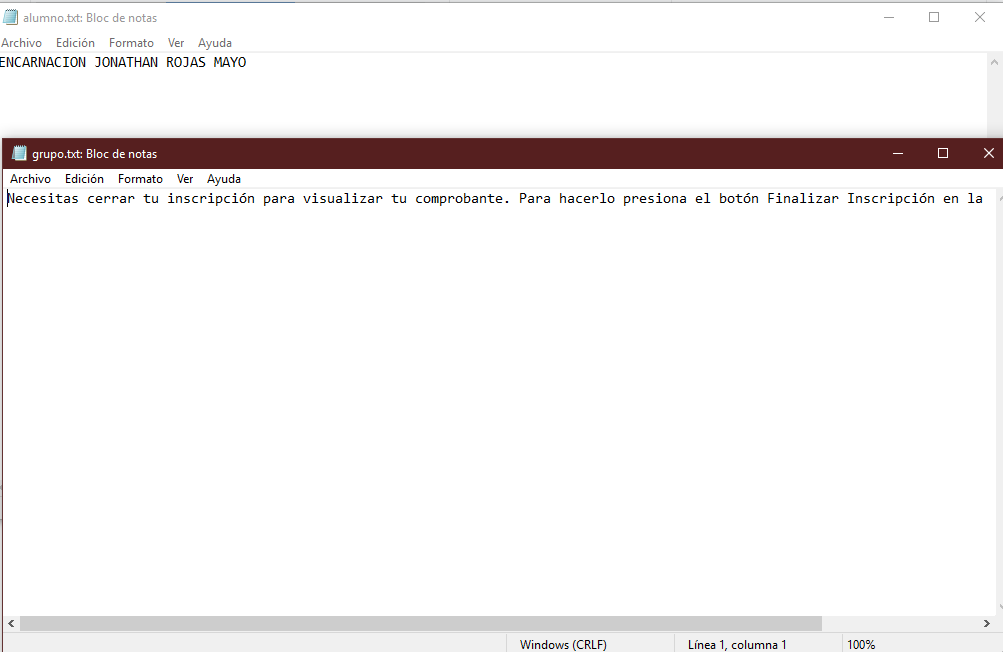
\includegraphics[width=10cm, height=6cm]{Imagenes/Crawler/Noinscrito}
		\caption{Respuesta del crawler.}
		\label{noinscrito}
	\end{figure}
	
	\noindent Se muestran las cadenas correspondientes a la extracción de información para validar que el alumno en cuestión esté inscrito o no lo esté.\\
	
	\textbf{POR EJEMPLO: CON USUARIO INSCRITO}\\
	\noindent Se inserta previamente la boleta y contraseña del alumno del SAES ESCOM.
	
	\begin{figure}[hbt!]
		\centering
		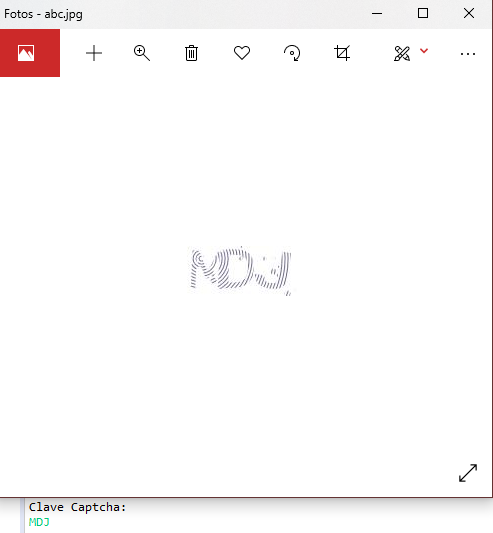
\includegraphics[width=10cm, height=6cm]{Imagenes/Crawler/Imagenlogininscrito}
		\caption{Captcha para el alumno inscrito.}
		\label{imagenlogininscrito}
	\end{figure}
	\noindent Se ingresa la clave captcha mostrada en la imagen “MDJ”
	\pagebreak
	
	\begin{figure}[hbt!]
		\centering
		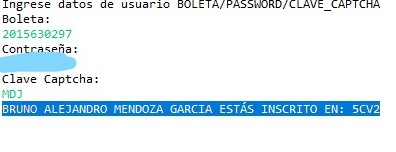
\includegraphics[width=10cm, height=6cm]{Imagenes/Crawler/Datoslogininscrito}
		\caption{Se registran ingresan datos al crawler.}
		\label{datoslogininscrito}
	\end{figure}
	
	\noindent Responde de acuerdo a la inscripción del alumno, para este caso el alumno ESTÁ INSCRITO.
	
	\begin{figure}[hbt!]
		\centering
		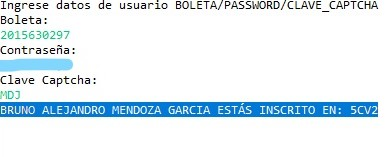
\includegraphics[width=10cm, height=6cm]{Imagenes/Crawler/Logininscrito}
		\caption{Respuesta del crawler.}
		\label{logininscrito}
	\end{figure}
	
	\begin{figure} [hbt!]
		\centering
		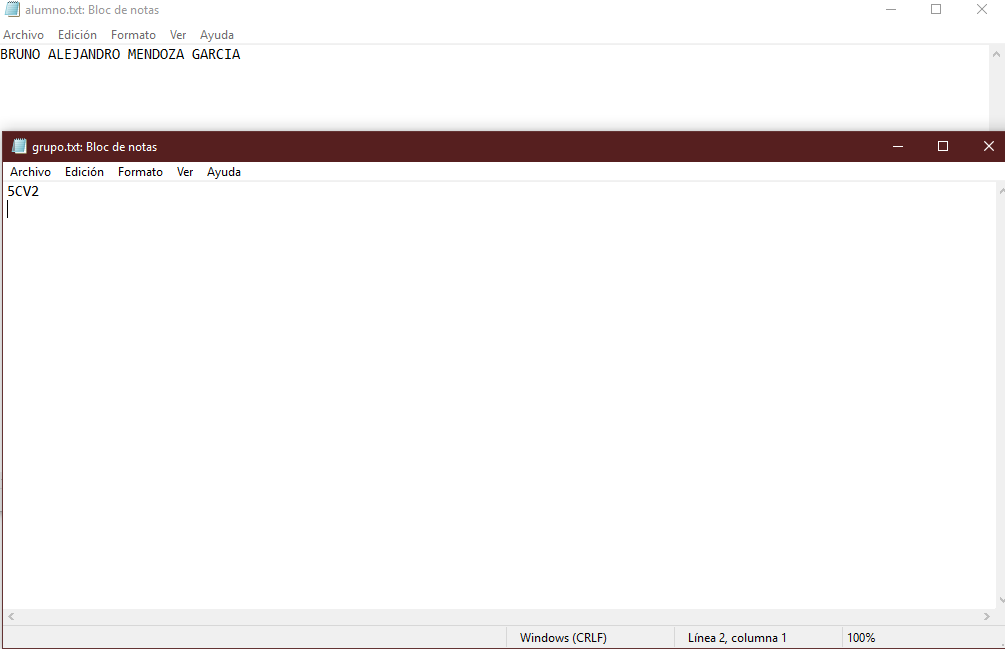
\includegraphics[width=10cm, height=6cm]{Imagenes/Crawler/Infologininscrito}
		\caption{Información del alumno inscrito.}
		\label{infologininscrito}
	\end{figure}
	\noindent Se muestran las cadenas correspondientes a la extracción de información para validar que el alumno en cuestión esté inscrito o no lo esté.
	
	
	%=========================================================
	%              Sistema Gestor de BD del lado del servidor
	%=========================================================
	\section{Sistema Gestor de Base de Datos del lado del servidor}
	\noindent Para persistir la información que se genere a través de la aplicación y que esté disponible la mayor parte del tiempo por los usuarios es necesario contar con un SGBD en el servidor para que los datos están centralizados y se puedan agregar, actualizar, consultar y eliminar los datos generados por los usuarios. Comparando los SGBD, ver la tabla 2, más populares encontramos que la opción más confiable será utilizar MySQL debido a que es de código abierto, gratuito, con soporte técnico y abundante documentación. 
	
	\begin{table}[htbp]
		\begin{center}
			\begin{tabular}{|l|p{35mm}|p{35mm}|p{35mm}|l}
				\hline
				Caracter\'isticas & Oracle & MySQL & SQL Server \\
				\hline 
				Interfaz & GUI, SQL & SQL & GUI, SQL \\ \hline
				Lenguaje soportado & C, C++, C, Java, Ruby y Objective-C & C, C, C++, D, Java, Ruby y Objective C & Java, Ruby, Python, VB, .Net y PHP  \\ \hline
				Sistema Operativo & Windows, GNU/Linux, Solaris, OS-X & Windows, GNU/Linux, OS-X, FreeBSD, Solaris & Windows \\ \hline
				Licencia & Propietrio & Código Libre & Propietario \\ \hline
			\end{tabular}
			\caption{Tabla comparativa de lenguajes de BD.}
			\label{tablaServidor}
		\end{center}
	\end{table}
	
	
	%=========================================================
	%                                                         Servidor
	%=========================================================

	\section{Servidor}
	\noindent Para establecer las caracteristicas de nuestro servidor debemos conocer parte de sus componentes y que operabilidad tendrá dedicada.
	Empezando con los procesadores dedicados para equipos de servidores, se recomienda usar Intel Xeon (cualquier versión), por ejemplo: los servidores con Intel Xeon E5 v3 pueden tener hasta 36 núcleos y se encuentran entre los pocos procesadores que son compatibles con la nueva versión DDR4 de RAM, que utiliza un consumo de energía muy reducido y brinda una excelente velocidad de transferencia de datos.\cite{serv}
	
	\noindent Tomando en cuenta las recomendaciones para armar un buen servidor se tomaron algunas caracteristicas de componentes que pueden ser accesibles para montar el proyecto. \cite{serv}\cite{servi}
	
	\begin{table}[htbp]
		\begin{center}
			\begin{tabular}{|l|l|}
				\hline
				\multicolumn{2}{|c|}{Servidor Ideal} \\
				\hline
				Componentes & \\
				\hline
				\multicolumn{2}{|c|}{Hardware} \\
				\hline
				Procesador & Intel Xeon ó AMD Opteron\\
				\hline
				Plataforma & 64-Bits\\
				\hline
				Memoria RAM & 8 GB\\
				\hline
				Disco Duro & 500 GB\\
				\hline
				Arreglo de Discos Duros & Ninguno\\
				\hline
				Monitor & 800 x 600 16 bits Color o Superior\\
				\hline
				\multicolumn{2}{|c|}{Software} \\
				\hline
				Sistema Operativo & Windows \\
				\hline
				Base de Datos & MySQL 5.1 Community Server\\
				\hline
			\end{tabular}
			\caption{Tabla de especificaciones del servidor.}
		\end{center}
	\end{table}
\pagebreak
\noindent Suponiendo el caso de que por día se hagan 1000 visitas diarias donde se tienen 6 páginas por visita que además por página consume 100kb.

\noindent En condiciones normales, una web envía más datos de los que recibe, por lo cual, hemos de contar con los datos enviados.
\\
\noindent Podremos calcular la transferencia de datos con la siguiente formula\\

(días por mes) x (visitas diarias) x (páginas por visita) x (volumen por página) x 1,25\\

\noindent En cuestión de la memoria RAM está esta pensada de manera que soporte las consultas realizadas por los usuarios en la aplicación, es bien dicho que entre más RAM el servidor tendrá mejor rendimiento \cite{servi}.

\noindent O bien Tomando como caso la capacidad del disco duro se considera que el almacenamiento no se saturará hasta pasado 1 año, puesto que el uso de memoria de almacenamiento de datos creados por la aplicación no serán concurrentes, con el proposito de almacenar la aplicación y los archivos de base de datos, cuya base de datos incrementa de acuerdo al número de usuarios que hagan uso de ella (unicamente los que estén inscritos, o usuarios coordinador).\\


%=========================================================
%                                             Reglas del sistema
%=========================================================
\section{Reglas del Sistema}
\noindent El alumno que desee participar en un evento interpolitécnico hará uso de la aplicación web RIDESCOM. Como primer punto deberá iniciar sesión en la misma, ingresando el usuario y contraseña con el que entra a sistema SAES (Sistema de Administración Escolar). Si los datos ingresados son correctos, se le dará acceso a la aplicación RIDESCOM, en caso contrario no se le dará acceso para poder registrarse en un evento. Sin embargo, podrá seguir visualizando datos generales, como lo es el calendario de eventos, resultados de eventos y los eventos que se practican dentro de la unidad académica.
El Jefe de Fomento Deportivo podrá dar de alta a un Coordinador de alguna Unidad Académica. Para dar de alta un evento deportivo deberá llenar todos los campos requeridos, tendrá la opción de agregar una descripción si así lo desea. 
El Coordinador de la Unidad Académica registrará a los entrenadores de las actividades deportivas deberá llenar los campos requeridos para poder concluir el registro. En caso de que exista un entrenador ya haya sido registrado, la aplicación le notificará. Una vez concluido los eventos deportivos, este registrará los resultados obtenidos por los participantes para que puedan ser vistos por la comunidad en general. 

%=========================================================
%                                             Reglas de Negocio
%=========================================================
\section{Reglas de Negocio}
\noindent La aplicación RIDESCOM permitirá a los alumnos que estén inscritos en el periodo actual, inscribirse en un evento interpolitécnico, consultar los eventos registrados, consultar calendario de eventos. 
El sistema cuenta con una interfaz que nos permite visualizar las diferentes opciones ofrecidas por el mismo. Para acceder al anterior el usuario debe de tener un usuario y contraseña. Dicho usuario y contraseña, será con el que ingresa al sistema del SAES. 
Así mismo, habrá “usuarios encargados”, quienes se encargan de controlar y supervisar el uso de éste ante pequeñas porciones de estudiantes (grupos de alumnos). Ahora dichos encargados hay dos tipos el Jefe de Fomento Deportivo, a este se le permitirá crear eventos deportivos, registrar eventos deportivos y restablecer contraseña a los perfiles de los coordinadores. El segundo tipo de encargado es el Coordinador de una Unidad Académica, este podrá registrar los resultados de los participantes en el sistema para poder ser visualizados en la vista principal, podrá generar un reporte de los alumnos registrados durante el periodo que se haya especificado y registrar a los entrenadores que laboran dentro de la Unidad Académica a la que atienda, a continuación se describirán las reglas para cada uno de los actores que se involucran.
\pagebreak


%=========================================================
%                                             Reglas de Negocio del JFD
%=========================================================
\section{Reglas de Negocio Jefe de Fomento Deportivo}
Para que el JFD pueda ingresar a la página RIDESCOM debe de contar con un Usuario y Contraseña, de caso contrario no podrá acceder.
Una vez dentro de la página de RIDESCOM se le mostrarán las opciones que tiene permitidas, tales como: Evento, Coordinadores, Usuarios, Pruebas en estos dos podrá agregar, editar o eliminar.

\noindent Para la vista de Evento, la información se le mostrará en la página principal, si hay eventos registrados estos serán mostrados en la tabla correspondiente, sino se cuenta con datos se mostrará en la tabla el mensaje de que no existen datos.  Para poder agregar un evento se deben de cumplir con algunos campos que son requisito sino se completan los campos no podrá registrar el evento.  Dentro del formulario para crear el evento se debe asignar una fecha en la que los alumnos podrán inscribirse para esto, no debe de ser mayor  a 5 días en la que se realizará el evento. También se debe considerar que no se puede asignar una fecha menor respecto a la fecha en que se está creando el evento. Una vez tenga el evento registrado podrá editar información respecto a este, teniendo en cuenta los campos que son requisito, o en caso contrario eliminar el evento.

\noindent Para la vista de Coordinadores, se mostrará la información en una tabla dentro de la página principal, en caso de no contar con datos registrados se mostrará un mensaje de que no existen datos. Para poder agregar un Coordinador de Unidad Académica deberá cumplir con campos que son requisitos sino se completan los campos no podrá registrar el coordinador. Una vez tenga el coordinador registrado podrá editar información respecto a este, teniendo en cuenta los campos que son requisito, o en caso contrario eliminar los datos del coordinador.

\noindent Contará con un apartado en el que visualizará los resultados obtenidos por los participantes estos estarán disponibles hasta que concluyan los eventos interpolitécnios y para el JFD solo será de consulta.

\noindent Para la vista de Pruebas, se mostrará una tabla en la que podrá ver las pruebas registradas, en caso de no tener datos que mostrar se mostrará un mensaje en el que se indique que no hay datos por mostrar. Se podrá agregar pruebas, para ello deberá de cumplir con los campos que son requisitos. De igual manera tendrá campos que son requisito para poder guardar los datos. Una vez guardado las Pruebas podrá editar o eliminar la información.

%=========================================================
%                                             Reglas de Negocio del Coord
%=========================================================
\section{Reglas de Negocio Coordinador de Unidad Académica}
\noindent Para que el Coordinador de Unidad Académica pueda ingresar a la página RIDESCOM debe de contar con un Usuario y Contraseña, de caso contrario no podrá acceder.\\

\noindent Una vez dentro de la página de RIDESCOM se le mostrarán las opciones que tiene permitidas, tales como: Constancias, Calendario, Resultados, Consulta Inscritos, DIfundir Evento y Entrenadores. Las vistas antes mencionadas exceptuando Resultados y Difundir Evento, serán vistas de solo lectura.\\

\noindent Para la vista de Constancias el Coordinador de la Unidad Académica podrá consultar si el alumno participó en un evento para que posteriormente, él pueda comenzar el trámite correspondiente para la generación de la constancia. Será solo vista de consulta/lectura. Para la vista de Calendario, se mostrará en la página principal del Coordinador una tabla con los datos que le corresponden, en caso de no tener información se mostrará el mensaje de que no existen datos. Esta vista sólo será de lectura.\\

\noindent Para la vista de Resultados el Coordinador de la Unidad Académica podrá visualizar la información en una tabla dentro de la página principal, en caso de no tener datos se mostrará el mensaje de que no existen datos Para ingresar los resultados obtenidos de los participantes, como el tiempo que se obtuvo, el lugar, etc., deberá de llenar los campos que son requisitos, sino se completan los campos no podrá registrarse el evento. Una vez que se tengan los datos registrados podrá editar o eliminar estos.\\

\noindent Para la vista Difundir Evento, el Coordinador de la Unidad Académica podrá visualizar los eventos que han sido registrados, al selecciona la opción difundir se le mostrará la opción de difundirlo en la red social de facebook.\\

\noindent Para la vista de Entrenadores, se mostrará la información dentro de la vista principal en una tabla, en caso de no contar con información se mostrará el mensaje de que no existen datos. Para agregar datos de un Entrenador se deben de cumplir con datos que son requisitos. Una vez que se tengan datos registrados podrá editar o eliminar la información. \\

\section{Reglas de Negocio Alumno}
Para que el alumno pueda ingresar a la página RIDESCOM debe de contar con un Usuario y Contraseña, de caso contrario no podrá acceder.\\

Una vez dentro de la página de RIDESCOM se le mostrarán las opciones que tiene permitidas, tales como: Calendario, Inscribe Interpolitecnico, Historial,  Resultados, Eventos Inscritos. Las vistas antes mencionadas serán solo lectura exeptuando la vista de INscribe Interpolitecnico.\\

Para la vista de Calendario se mostrará en la página principal en una tabla que contenga la información, en caso de que esta no cuente con información se mostrará el mensaje de que no existen datos. Esta vista sólo será de lectura para el alumno.\\

Para la vista de Inscribir Interpolitecnio, el alumno pueda inscribir un Evento Interpolitecnico deberá como primer punto, validar su status académico, para ello se le mostrará en segunda ocasión el inicio de sesión con esto, se verificará su estatus académico. Si el alumno está inscrito entonces se le mostrará una segundo vista en la que solo será de lectura y verificará si sus datos son correctos. En caso de que el alumno no esté inscrito se le mostrará un mensaje para notificarle que no puede inscribirse dado que no está inscrito en el periodo actual. \\
Si la información que se le presenta es correcta podrá continuar para seleccionar el evento en el que desea participar y así concluir con su inscripción. \\

Para la vista Historial, se mostrará al alumno una tabla que le proporcione información de los eventos en los que ha participado a lo largo de su trayectoria académica. Esta vista es de solo lectura.\\

Para la vista Resultado, se mostrará la información de los resultados del último evento en el que a participado. Esta vista es de solo lectura.\\

Para la vista de Eventos Inscritos, mostrará el o los eventos a los que se a registrado el alumno en el periodo en curso. Esta vista es de solo lectura.\\

\noindent A continuación se mostrarán en distintas tablas las Reglas de Negocio de acuerdo a cada actor que involucra la aplicación.

\begin{table}[hbt!]
	\begin{center}
		\begin{tabular}{|p{30mm}|p{100mm}|}
			\hline
			\multicolumn{2}{|c|}{Jefe de Fomento Deportivo} \\
			\hline
			Identificador & Descripción \\
			\hline 
			RN 1 & Para ingresar a la página debe de contar con un usuario y contraseña. \\ \hline
			RN 2 &  Para registrar un nuevo evento deben de completarse todos los campos que son requisito.\\ \hline
			RN 3 & Para registrar un evento debe de considerar que la fecha de este no sea menor a la fecha en la que se quiere realizar el mismo (no debe de ser mayor  a 5 días en la que se realizará el evento). \\ \hline
			RN 4 &  La fecha de inicio de registro para los alumnos no rebase la fecha en la que se realizará el evento.\\ \hline
			RN 5 &  La fecha de fin de registro para los alumnos no rebase la fecha en la que se realizará el evento. \\ \hline
			RN 6 & Para editar los datos de un evento, no debe de haber alumnos inscritos. \\ \hline
			RN 7 &  Al editar los datos de un evento debe considerar completar todos los campos.\\ \hline
			RN 8 &  Para eliminar un evento, no debe de haber alumnos inscritos en este.\\ \hline
			RN 9 &  Para agregar un deporte, todos los campos que son requisito deben completarse.\\ \hline
			RN 10 &  Al editar un deporte, se debe considerar completar todos los campos requeridos.\\ \hline
			RN 11 &  Para registrar una Prueba, se debe de completar todos los campos.\\ \hline
			RN 12 & Al editar los datos se debe considerar completar todos los campos.\\ \hline
			RN 13 &  Al registrar un nuevo Coordinador, se debe asignar un usuario y contraseña.\\ \hline
			RN 14 &  Para completar el registro, debe completarse todos los campos requeridos.\\ \hline
			RN 15 &  Al editar los datos de un Coordinador, se debe tomar en cuenta completar todos los campos requeridos.\\ \hline
			RN 16 &  Para registrar una Sede, deben completarse todos los campos requeridos.\\ \hline
			RN 17 &  Al editar los datos de una Sede, se debe considerar que esta no esté asignada en un evento.\\ \hline
		\end{tabular}
		\caption{Reglas de Negocio Jefe de Fomento Deportivo.}
		\label{RNJFD}
	\end{center}
\end{table}

\begin{table}[hbt!]
	\begin{center}
		\begin{tabular}{|p{30mm}|p{100mm}|}
			\hline
			\multicolumn{2}{|c|}{Coordinador de Unidad Acedémica} \\
			\hline
			Identificador & Descripción \\
			\hline 
			RN 18 &  Para ingresar a la página debe de contar con un usuario y contraseña.\\ \hline
			RN 19 & Las credenciales deben estar activas y ser proporcionadas por el Jefe de Fomento Deportivo.\\ \hline
			RN 20 & Para ingresar los resultados, debe seleccionar un usuario. \\ \hline
			RN 21 & Se debe seleccionar una prueba correspondiente al alumno.\\ \hline
			RN 22 & Para terminar el proceso de registro de resultados, debe completar los campos requeridos. \\ \hline
			RN 23 & Para registrar un entrenador debe llenar todos los campos requeridos.\\ \hline
			RN 24 & Para obtener la cédula de inscripción, el coordinador deberá de seleccionar el tipo de deporte, así como el ciclo escolar. \\ \hline
			RN 25 & Para consultar si un alumno participó en un evento, se debe buscar por medio de su boleta o por el ciclo escolar en el que participó.\\ \hline
			RN 26 & Para difundir un evento, deberá seleccionar el evento de la tabla y seleccionar el medio por el cual quiere compartir el evento.\\ \hline
		\end{tabular}
		\caption{Reglas de Negocio Coordinador de Unidad Académicas.}
		\label{RNCUA}
	\end{center}
\end{table}

\pagebreak

\begin{table}[hbt!]
	\begin{center}
		\begin{tabular}{|p{30mm}|p{100mm}|}
			\hline
			\multicolumn{2}{|c|}{Alumno} \\ \hline
			Identificador & Descripción \\ \hline 
			RN & Para ingresar a la página debe de contar con un usuario y contraseña.\\ \hline
			RN & El alumno debe verificar el estatus académico para poder registrarse en un evento.\\ \hline
			RN & Para concluir el registro al evento, debe de llenar todos los campos requeridos.\\ \hline
			RN & Puede inscribirse en los eventos que desee, siempre y cuando no tenga traslape en horas de los eventos.\\ \hline
			RN & \\ \hline
			RN & \\ \hline
		\end{tabular}
		\caption{Reglas de Negocio para el alumno.}
		\label{RNA}
	\end{center}
\end{table}
\pagebreak

%=========================================================
%                                                         Requisitos de interaccion con el usuario
%=========================================================
\section{Requisitos del usuario}
A continuación se mostrarán los requisitos indispensables que se deben considerar para el usuario, así como la prioridad de cada uno de ellos. Estos servirán para el desarrollo de los módulos que conformarán la aplicaciónweb 
\begin{table}[htbp]
	\begin{center}
		\begin{tabular}{|l|p{45mm}|p{45mm}|p{45mm}|l}
			\hline
			Id & Nombre & Descripción & Prioridad \\
			\hline 
			RF1 & Registro de eventos & En la aplicación web se podrán registrar, modificar, eliminar y consultar  en un formulario todos los datos para identificar un evento.
			& MEDIA \\ \hline
			RF2 & Registro de participantes & En la aplicación web se podrán registrar, modificar, eliminar y consultar  en un formulario los datos del participante & ALTA  \\ \hline
			RF3 & Vista al público & En una pantalla se mostrarán los participantes que estén registrados en la aplicación y ver sus resultados de competencia. & MEDIO \\ \hline
			RF4 & Conexión con red social FACEBOOK. & Gracias a los datos que identifican a un evento se podrá promover en la red social FACEBOOK mediante el uso de API.& ALTA \\ \hline
			RF5 & Realizar una interfaz para los participantes (alumnos). &Se creará un(una ventana)  sitio para los alumnos que quieran participar en algún evento deportivo(, haciendo su registro, consultar estatus). & MEDIA \\ \hline
			RF6 & Mostrar una tabla de estadísticas. & En una pantalla (vista)  se mostrará todas las áreas deportivas que participaron en el evento deportivo y  número de participantes. & ALTA \\ \hline
			RF7 & Registrar un coordinador & El coordinador que utilizará la aplicación web tendrá que ser registrado en la base de datos. & ALTA \\ \hline
			RF8 & Vista para el coordinador. &El coordinador tendrá una vista donde podrá dar de alta eventos, participantes y generar cédulas de inscripción. & MEDIA \\ \hline
			RF9  & Historial & Para que se tenga un monitoreo de participantes. & ALTA \\ \hline
		\end{tabular}
		\caption{Requerimientos del Usuario.}
		\label{tabla:sencilla}
	\end{center}
\end{table}
\pagebreak

%=========================================================
%                                                         Requisitos funcionales
%=========================================================
\section{Requisitos funcionales de la aplicación web}
En la tabla mostrada a continuación, se muestrán los requisitos funcionales de la aplicación web los cuales serviran para el desarrollo de la aplicación web, así como la prioridad de cada uno de ellos.
\begin{table}[htbp]
	\begin{center}
		\begin{tabular}{|l|p{45mm}|p{45mm}|p{45mm}|l}
			\hline
			Id & Nombre & Descripción & Prioridad \\
			\hline 
			RF1 & Conexión a internet. & La aplicación deberá estar siempre conectada a internet & ALTA \\ \hline
			RF2 & Validación de datos de los participantes. & La aplicación contará con un mecanismo de comprobación de estado académico (inscrito). & ALTA \\ \hline
			RF3 & Historial de participante. & Para tener seguimiento del participante durante su trayectoria académica & MEDIA  \\ \hline
			RF4 & Comunicación con la red social FACEBOOK &Habrá comunicación con la red social FACEBOOK para la publicación de eventos registrados en la aplicación.  & MEDIO \\ \hline
			RF5 & Creación de perfiles. & Se podrá asignar un perfil a un usuario.& MEDIA \\ \hline
		\end{tabular}
		\pagebreak
		\caption{Requerimientos funcionales de la aplicación web.}
		\label{tabla:sencilla}
	\end{center}
\end{table}


%=========================================================
%                                                         Requisitos de informacion
%=========================================================
\section{Requisitos no funcionales de la aplicación web}
En la tabla mostrada a continuación se muestran los requisitos que no afectan al funcionamiento de la aplicación, sin embargo se consideran para que en caso de tener el tiempo, se integran a la aplicación y obtener un complemento al resultado fijado.
\begin{table}[htbp]
	\begin{center}
		\begin{tabular}{|l|p{45mm}|p{45mm}|p{45mm}|l}
			\hline
			Id & Nombre & Descripción & Prioridad \\
			\hline 
			RF1 & Vista de consulta genera. & Comunidad ajena a los participantes podrán ver los resultados. & MEDIA \\ \hline
			RF2 & Lista de registros &El usuario podrá consultar sus registros realizados & MEDIA   \\ \hline
			RF3 & Recuperación de contraseña &El usuario participante podrá recuperar su contraseña. & MEDIO \\ \hline
		\end{tabular}
		\caption{Requerimientos no funcionales de la aplicación web.}
		\label{tabla:sencilla}
	\end{center}
\end{table}
\pagebreak

%=========================================================
%                                    Diagrama de procesos
%=========================================================
\section{Diagrama de Procesos}
\noindent En este apartado se explicará y detallará el proceso actual que sigue el alumno para poder registrarse en un evento interpolitécnico deportivo, posteriormente se hace mención del proceso porpuesto para el mismo fin.\\
El proceso actual que el alumno debe seguir para inscribirse a un evento interpolitécnico deportivo comienza cuando el alumno acude al Deportamento de Actividades Deportivas de su unidad académica donde el encargado del departamento le proporciona un formato el cual debe llenar a mano. Este formato se debe de llenar de acuerdo al número de eventos en el que el alumno quiera participar.\\
El formato antes mencionado solicita campos como: nombre, deporte, escuela, prueba, entre otros. Una vez completado el formato el alumno entrega su solicitud al encargado del Departamento y este hace mención que se comunicarán con el en cuanto se tenga una actualización acerca de su solicitud.\\
\noindent El proceso continua con el encargado del Departamento de Actividades Deportivas quien genera una lista de alumnos solicitantes para posteriormente comprobar su estatus académico. Esto se realiza ya que según el reglamento solo los alumnos participantes son los que pueden participar en los eventos.
Una vez que realizada la comprobación se le notifica al alumno el estatus final de su solicitud, sea aceptada o rechazada.
El coordinador de la unidad académica realiza un listado con los alumnos que participaran en los eventos de acuerdo al ciclo escolar en curso para que sea enviado al Departamento de Fomento Deportivo.
Finalmente el alumno espera a que sea la fecha del evento para hacer su participación. Una vez concluido estos, se procede a pagar el arbitraje que se contrata para llevar control de las actividades deportivas.\\
\noindent Una vez pagado el arbitraje se pasa a hacer el llenado de los resultados obtenidos para cada uno de los participantes para así ser publicados y pueda ser visualizados por la comunidad estudiantil.


%=========================================================
%                                                         Reglas de Negocio del Sistema
%=========================================================
%\section{Reglas de necocio de la aplicación}


\section{Diseño de pantallas}}
\noindent Las vistas han cambiado conforme avanza el proyecto, en este caso, se han omitido unas vistas ya que durante nuestra investigación para implementar el registro a la página RIDESCOM para los alumnos, en un inicio se planteo hacer una conexión con la base de datos de la Dirección de Administración Escolera (DAE) para poder verificar que sus datos sean reales. Este método de comprobación iba a ser difícil de llevar a cabo ya que por el hecho de manejar datos sensibles no se nos podía ser brindada. Por esta razón se investigo como poder implementar un crawler, que se conecta con el SAES. Dentro de la página RIDESCOM se solicitan los mismos campos que en el SAES: Usuario, Contraseña y Captcha, si los datos que se ingresaron son correctos el alumno podrá ingresar a RIDESCOM, en caso contrario se le notificará que los datos son erróneos. \\
Las vistas que se eliminaron son las siguientes: 

\begin{figure}[hbt!]
	\centering
	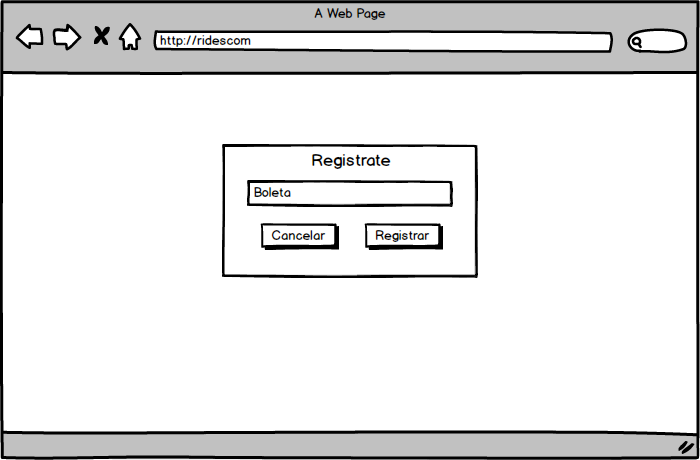
\includegraphics[width=10cm, height=6cm]{Imagenes/Disenos/VistasBorradas/p1_Registro.png}
	\caption{Registro para los alumnos.}
\end{figure}

\begin{figure}[hbt!]
	\centering
	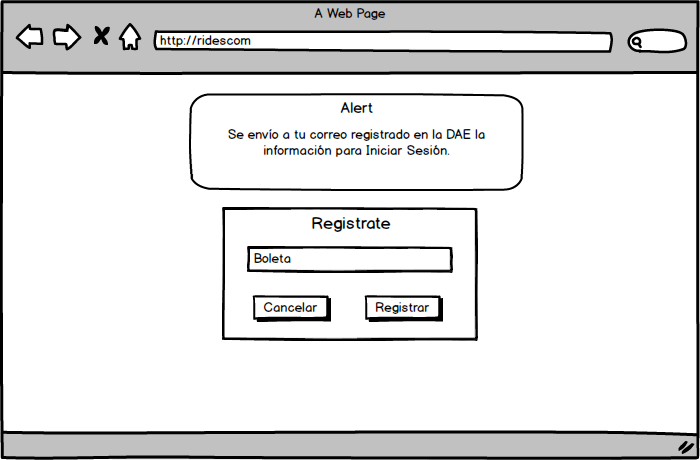
\includegraphics[width=10cm, height=6cm]{Imagenes/Disenos/VistasBorradas/ConfirmacionRegistro.png}
	\caption{Confirmación registro para los alumnos.}
\end{figure}

\begin{figure}[hbt!]
	\centering
	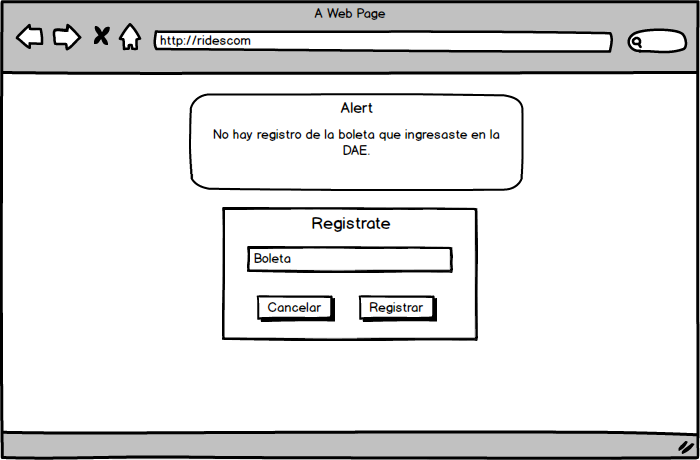
\includegraphics[width=10cm, height=6cm]{Imagenes/Disenos/VistasBorradas/p3RechazoRegistro.png}
	\caption{Rechazo registro para los alumnos.}
\end{figure}

\begin{figure}[hbt!]
	\centering
	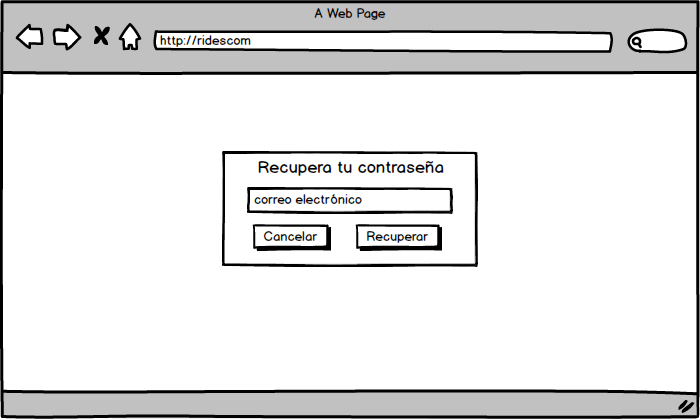
\includegraphics[width=10cm, height=6cm]{Imagenes/Disenos/VistasBorradas/p5Recuperarcontrasena.png}
	\caption{Recuperar contraseña para los alumnos.}
\end{figure}

\begin{figure}[hbt!]
	\centering
	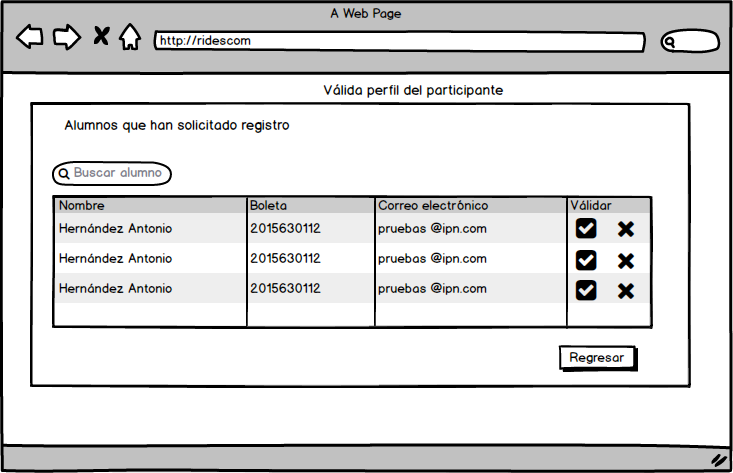
\includegraphics[width=10cm, height=6cm]{Imagenes/Disenos/VistasBorradas/p18ValidaPerfil.png}
	\caption{Validar perfil de los alumnos.}
\end{figure}
\pagebreak

